\section{Mathematische Grundlagen der Robotik}

\subsection{TI-Nspire CX CAS Befehle}
Die Bibliothk findet sich im Repo \href{LMazzole/tinspire}{https://github.com/LMazzole/tinspire}\newline
\begin{tabular}{p{5cm}p{10cm}}

\texttt{$[ x_{11} , x_{12} ; x_{21},x_{22}]$} &  $ \begin{bmatrix}
            	x_{11} & x_{12}\\
            	x_{21} & x_{22}\\
            \end{bmatrix} $ \\
\texttt{ $[ \ldots]^{-1} $} & Inverse Matrix\\
\texttt{ $[ \ldots] $ (2ND CATALOG) \small{T} } & Transponierte Matrix
$[\ldots]^{T}$\\

\end{tabular} \\
	
%
%	\subsection{Matritzenrechnen}
%		\subsubsection{Vektoren im Raum}
%			$\vec{p}_{AB}=
%			\begin{matrix}
%            	x_B-x_A\\
%            	y_B-y_A\\
%            	z_B-z_A\\
%            \end{matrix}$\\
%			
%			Transponierung: $a^T\cdot b= \left(a_1 \vspace{0.2cm} a_2\vspace{0.2cm}  \ldots a_n \right) 
%			\cdot $
%	
%		\subsubsection{Matrizen Multiplikation \small{(A muss gleich viele Spalten
%		haben wie B Zeilen hat)}}
%		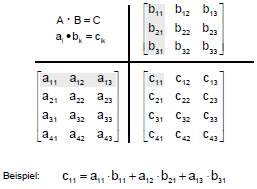
\includegraphics[width=7cm]{./bilder/matrizenmultiplikation.png}
%    	
%	
%	
%	
%\subsection{Übersicht}
%	\begin{tabular}{l l}
%    	Transponierte Matrix: & $A^T=[a_{ik}^T]=[a_{ki}]$ vertauschen der Zeilen
%    	mit Spalten\\
%    	Einheitsmatrix:& $I_n= 
%			    	\begin{bmatrix} 
%			        	1&0 & 0\\
%			        	0&1&0\\
%			        	0&0&1                               
%			        \end{bmatrix}$		    
%    \end{tabular}
%
\subsection{Determinante}
\begin{minipage}{9cm}
    
    	\textbf{2x2 Matrix}    
    $$ \det \begin{bmatrix} a_{11} & a_{12} \\
                            a_{21} & a_{22} \end{bmatrix} =
                            a_{11} a_{22} - a_{12} a_{21}  $$
\end{minipage}
\begin{minipage}{0.45\linewidth}
    	\textbf{3x3 Matrix}\newline
    $ \det \begin{bmatrix} a_{11} & a_{12} & a_{13} \\
    a_{21} & a_{22}& a_{23} \\
    a_{31} & a_{32} & a_{33} \end{bmatrix}
    $=\begin{minipage}{0.7\linewidth}
        $a_{11} a_{22} a_{33}
        + a_{12} a_{23} a_{31}
        + a_{13} a_{21} a_{32}$ \newline$
        - a_{13} a_{22} a_{31}
        - a_{12} a_{21} a_{33}
        - a_{11} a_{23} a_{32}  $
    \end{minipage} 
\end{minipage}	

%	
% 	\textbf{Dreiecksmatrix} - Alle Elemente entweder ober- oder unterhalt der Hauptdiagonale $= 0$
% 	$$\det A =a_{11}\cdot a_{22}\dotsb a_{nn} \quad  \quad \text{Die Det. ist das Produkt
% 	der Hauptdiagonal-Einträge. Gilt somit auch für Diagonalmatritzen.} $$
%% 	
%	\textbf{Null $(|A| = 0)$} - Wenn $A$ eine (n,n)-Matrix ist, so wird $|A| = 0$ unter einer der
%	folgenden Bedingungen:
%	\begin{itemize}
%    	\item Zwei Zeilen/Spalten sind linear abhängig (gleich oder ein Vielfaches der anderen).
%    	\item Alle Elemente einer Zeile/Spalte sind Null. \\
%  	\end{itemize} 
%	\clearpage
% 	\textbf{Allgemein:}
% 	$$A\epsilon M_n: \det A =    
% 	\begin{vmatrix}
%     	a_{11} & a_{12}& \ldots & a_{1n}\\
%     	a_{21}& &\ldots & \\
%     	\ldots \\
%     	a_{n1} & & \ldots & a_{nn}    			
%     \end{vmatrix}=
% 	(-1)^{1+1}a_{11}D_{11} + (-1)^{1+2}a_{12}D_{12}+ \ldots +
% 	(-1)^{1+n}a_{1n}D_{1n}$$
% 	
% 	\subsubsection{Unterdeterminante}
% 	$$D_{11}=
% 	\begin{vmatrix}
%     	a_{22} & \ldots & a_{2n}\\
%     	\ldots\\
%     	a_{n2}& \ldots & a_{nn}
%     \end{vmatrix} 	\\
% 	D_{12}=
% 	\begin{vmatrix}
%     	a_{21} & a_{23}& \ldots & a_{2n}\\
%     	\ldots\\
%     	a_{n1}& a_{n3}&\ldots & a_{nn}
%     \end{vmatrix}$$\\
% 	$D_{ij}$ die (n-1)$ \times $(n-1)-Untermatrix von D ist, die durch Streichen der
% 	i-ten Zeile und j-ten Spalte entsteht.\\
% 	Diese Methode ist zu empfehlen, wenn die Matrix in einer Zeile oder Spalte
% 	bis auf eine Stelle nur Nullen aufweisst.
% 	Dies lässt sich meist mit dem Gausverfahren bewerkstelligen.
% 	
% \subsection{Gaussverfahren}
% 	Durch Addition und Subtraktion einzelner Zeilen (auch von Vielfachen einer
% 	Zeile) werden einzelne Stellen auf Null gebracht. zB:\\
% 	$\begin{bmatrix}
%     	a_{11} & a_{12}& \ldots & a_{1n}\\
%     	a_{21}& &\ldots & \\
%     	\ldots \\
%     	a_{n1} & & \ldots & a_{nn}    			
%     \end{bmatrix}=
% 	\begin{bmatrix}
%     	a_{11} & a_{12}& \ldots & a_{1n}\\
%     	k a_{21}-n a_{11}& ka_{22}-n a_{12}&\ldots & k a_{2n} - n a_{1n}\\
%     	\ldots \\
%     	a_{n1} & & \ldots & a_{nn}    			
%     \end{bmatrix}$ \\
% 	Die n * erste Zeile wurde von der k * zweiten Zeile abgezogen ($a_{2.}= 
% 	k a_{2.}- n a_{1.}$) 
	
\subsection{Inverse Matrix}
Existiert nur wenn Matrix regulär: $\det A \neq 0$\newline
\begin{minipage}{9cm}
	\textbf{2x2 Matrix}
	$$ A^{-1} = \begin{bmatrix} a & b \\ c & d \\ \end{bmatrix}^{-1} = \frac{1}{ad
	- bc} \begin{bmatrix} d & -b \\ -c & a \\ \end{bmatrix} $$
\end{minipage}
\begin{minipage}{11cm}
	\textbf{3x3 Matrix}\newline
  $  A^{-1} = \begin{bmatrix} a & b & c\\ d & e & f \\ g & h & i \\ \end{bmatrix}^{-1} =
  \frac{1}{\det(A)} \begin{bmatrix} ei - fh & ch - bi & bf - ce \\ fg - di & ai
  - cg & cd - af \\ dh - eg & bg - ah & ae - bd \end{bmatrix} $
\end{minipage}\\

% \textbf{Diagonalmatrix} (Alle Elemente ausserhalb der Hauptdiagonale $= 0$, Elemente auf
% Hauptdiagonale sind Eigenwerte $\lambda_i$): \\ 
% Alle Elemete elementweise invertieren - Kehrwert. $\quad \Rightarrow \quad $\textit{Gilt nur wenn
% alle Elemente auf der Hauptdiagonale $\neq 0$ sind.}\\
% 
% \textbf{Allgemein:}\\
% 	$A^{-1}= \begin{bmatrix}
%     	a_{11} & a_{12}& \ldots & a_{1n}\\
%     	a_{21}& &\ldots & \\
%     	\ldots \\
%     	a_{n1} & & \ldots & a_{nn}    			
%     \end{bmatrix}^{-1}$
% 	\begin{enumerate}
% 		\item $A^T$ bestimmen (Zeilen und Spalten vertauschen) $A^{T}= \begin{bmatrix}
%     	a_{11} & a_{21}& \ldots & a_{n1}\\
%     	a_{12}& &\ldots & \\
%     	\ldots \\
%     	a_{1n} & & \ldots & a_{nn}    			
%     \end{bmatrix}$	
% 		\item Bei $A^T$ jedes Element $a_{ij}$ durch Unterdet. $D_{ij}$ mit
% 		richtigem Vorzeichen ersetzen $A^*=	\begin{bmatrix}
% 			(-1)^{1+1}D_{11} &  \ldots	& (-1)^{1+n} D_{1n}\\
% 			\ldots\\
% 			(-1)^{n+1} D_{n1}& \ldots  & (-1)^{n+n} D_{nn}
% 		\end{bmatrix}$
% 		\item $A^{-1} = \frac{A^*}{\det A}$ 
%     \end{enumerate}
%  
%  \subsection{Diagonalisierung}
%  	\begin{enumerate}
%        \item Eigenwerte $\lambda$ auschrechnen: $\det (A - I_n \lambda)=0$
%        \item Eigenvektoren $\vec{v}$ bilden: $(A- \lambda I_n)\vec{v}=0$
%        \item Transformationsmatrix: $T= [\vec{v_1} \ldots \vec{v_n}]$
%        \item $T^{-1}$ berechnen (Achtung ist A symmetrisch, dh. $A^T=A$ und
%        oder alle EV senktrecht zueinander, dann $T^{-1}=T^T$)
%        \item $D=\begin{bmatrix}
%                 	\lambda_1 &0 &0\\
%                 	0& \lambda_2 &0\\
%                 	0& 0& \lambda_3
%                 \end{bmatrix}$
% 		\item $A^n = T D^n T^{-1}$
% 
%      \end{enumerate}
\subsection{Basis Rotationsmatrizen}
Der Winkel ist Positiv bei einer Rotation im Gegenuhrzeigersinn $ \circlearrowleft $\newline
	\begin{minipage}{0.33\linewidth}
		Rotation um x-Achse mit Winkel $\gamma$ \\
   		$R_x(\gamma)=\begin{bmatrix}
                		1 &0 &0\\
                		0 &cos(\gamma) &-sin(\gamma)\\
                		0 &sin(\gamma) &cos(\gamma)
                	 \end{bmatrix}$
    \end{minipage}
	\begin{minipage}{0.33\linewidth}
    	Rotation um y-Achse mit Winkel $\beta$\\
   		$R_y(\beta)=\begin{bmatrix}
                		cos(\beta) &0 &sin(\beta)\\
                		0 &1 &0\\
                		-sin(\beta) &0 &cos(\beta)
                	 \end{bmatrix}$
    \end{minipage}
	\begin{minipage}{0.33\linewidth}
    	Rotation um z-Achse mit Winkel $\alpha$ \\
   		$R_z(\alpha)=\begin{bmatrix}
                		cos(\alpha) &-sin(\alpha) &0\\
                		sin(\alpha) &cos(\alpha) &0\\
                		0 &0 &1
                	 \end{bmatrix}$
    \end{minipage}
\subsection{Aufeinanderfolgende Rotationen}
3 Koordinatensysteme \{A\}, \{B\}, \{C\} mit gleichem Ursprung\\ \\
\begin{minipage}{6cm}
    \textbf{Körperfestkoordinatensystem}\\
    "`An der Achse"'\\
    ${}^B\mathrm{p}={}^B_C\mathrm{R}\cdot{}^C\mathrm{p}$\\
    ${}^A\mathrm{p}={}^A_B\mathrm{R}\cdot{}^B\mathrm{p}$\\
    ${}^A\mathrm{p}={}^A_C\mathrm{R}\cdot{}^C\mathrm{p}$\\ \\
    ${}^A_C\mathrm{R}=\overrightarrow{{}^A_B\mathrm{R} \cdot {}^B_C\mathrm{R}}$\\
\end{minipage}
\begin{minipage}{6cm}
    \textbf{Raumfestkoordinatensystem}\\ 
    "`An der Welt oder Basis"'\\
    ${}^B\mathrm{p}={}^B_A\mathrm{R}{}^B_C\mathrm{R}{}^A_C\mathrm{R}\cdot{}^C\mathrm{p}$\\
    ${}^A\mathrm{p}={}^A_B\mathrm{R}\cdot{}^B\mathrm{p}$\\
    ${}^A\mathrm{p}={}^A_C\mathrm{R}\cdot{}^C\mathrm{p}$\\ \\
    ${}^A_C\mathrm{R}=\overleftarrow{{}^B_C\mathrm{R} \cdot {}^A_B\mathrm{R}}$\\
\end{minipage}   

\subsubsection{Punkte in verschiedenen Koordinatensystemen \robo{36}{2.1.6}}
\begin{tabular}{ll}
    \textbf{Translation}&${}^A\mathrm{P} = {}^A\mathrm{P}_{OB}+{}^B\mathrm{P} $ \\
    \textbf{Rotation} & ${}^A\mathrm{P} = {}^A_B\mathrm{R}\cdot {}^B\mathrm{P} $\\
    \textbf{Rotation + Translation}&$ {}^A\mathrm{P} = {}^A\mathrm{P}_{OB} +{}^A_B\mathrm{R}\cdot {}^B\mathrm{P} $\\
\end{tabular}
\clearpage


\subsection{Konvention Arctan2 \robo{42}{2.1.8}}
	\begin{minipage}{10cm}
    	$\theta=\arctan2(y,x)\Longrightarrow\left\{
    	\begin{array}{l}
            \text{1:\space\space}\theta=\arctan(\frac{y}{x})\\
			\text{2:\space\space}\theta=\pi+\arctan(\frac{y}{x})\\
			\text{3:\space\space}\theta=-\pi+\arctan(\frac{y}{x})\\
			\text{4:\space\space}\theta=-\arctan(\frac{y}{x})\\
		\end{array}\right.$
    \end{minipage}
	\begin{minipage}{10cm}
    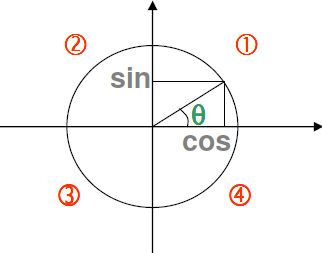
\includegraphics[width=4cm]{./bilder/einheitskreis.png}
    \end{minipage}

	\begin{minipage}{5cm}
    	\vspace{9mm}
    	$\theta=arctan2(\overbrace{y}^{sin(\theta)},\overbrace{x}^{cos(\theta)}) \Leftrightarrow$
    \end{minipage}
	\begin{minipage}[t]{0.8cm}
    	\textcircled{1}\\
    	\textcircled{2}\\
    	\textcircled{3}\\
    	\textcircled{4}
    \end{minipage}
	\begin{minipage}[t]{3.5cm}
    	$\theta= arctan(\frac{y}{x})$\\
    	$\theta= \pi + arctan(\frac{y}{x})$\\
    	$\theta= -\pi + arctan(\frac{y}{x})$\\
    	$\theta= -arctan(\frac{y}{x})$\\
    \end{minipage}
	\begin{minipage}[t]{2.5cm}
    	\hspace{2mm} $0 \leq \theta \leq \frac{\pi}{2}$\\
    	\hspace*{1.5mm} $\frac{\pi}{2} \leq \theta \leq \pi$\\
    	$-\pi \leq \theta \leq -\frac{\pi}{2}$\\
    	$-\frac{\pi}{2} \leq \theta \leq 0$
    \end{minipage}
	\begin{minipage}[t]{2.5cm}
    	für $+y$, $+x$\\
    	für $+y$, $-x$\\
    	für $-y$, $-x$\\
    	für $-y$, $+x$
    \end{minipage}
	\begin{minipage}[t]{4cm}
     	\begin{tabular}[t]{|l}
    	$\theta = \frac{\pi}{2}$ für $x=0$, $y>0$\\
    	$\theta = - \frac{\pi}{2}$ für $x=0$, $y<0$\\
    	$\theta = 0$ für $x=0$, $y=0$\\
    	\end{tabular}
    \end{minipage}

Ti Nspire CX CAS: \texttt{$ lm\backslash arctan2(Y,X)$}
\clearpage

\subsection{Rücktransformation auf Winkel}
	\begin{minipage}{9.5cm}
    \subsubsection{Z-Y-X Euler Winkel \robo{42}{2.1.8}}
    \begin{tabular}{|p{2.5cm}|p{6cm}|}
        \hline
        \multicolumn{2}{|l|}{Körperfest Koordinatensystem}\\
        \hline
        Vorgehen&
        \vspace{-0.3cm}
        \begin{enumerate}
            \item Drehen um Z mit Winkel $\alpha$
            \item Drehung um Y' mit Winkel $\beta$
            \item Drehung um X'' mit Winkel $\gamma$\vspace{-0.5cm}
        \end{enumerate}\\
        \hline
        Rotationsmat.:
        & ${^A_B}R(\overrightarrow{\alpha,\beta,\gamma}) = 
        \begin{bmatrix} 
        r_{11} & r_{12} & r_{13} \\
        r_{21} & r_{22} & r_{23} \\
        r_{31} & r_{32} & r_{33}                              
        \end{bmatrix}$ \\
        \hline
        \multicolumn{2}{|l|}{{\footnotesize 
                $ \overrightarrow{R_Z(\alpha)\cdot R_{Y'}(\beta) \cdot R_{X''}(\gamma)}$= $\begin{bmatrix} 
                c\alpha c\beta & c\alpha s\beta s\gamma - s\alpha c\gamma & c\alpha s\beta c\gamma + s\alpha s\gamma \\
                c\alpha c\beta & s\alpha s\beta s\gamma + c\alpha c\gamma & s\alpha s\beta c\gamma - c\alpha s\gamma \\
                -s\beta & c\beta s\gamma & c\beta c\gamma                            
                \end{bmatrix}$
        }}\\\hline 
        \multicolumn{2}{|l|}{\textbf{Rücktransformation}}\\
        \hline
			Ansatz:
& $cos(\beta) = \sqrt{r^2_{11} + r^2_{21}}$ \\
& $sin(\beta) = -r_{31}$\\
\hline
Winkel:
& $\beta=arctan2(-r_{31},\sqrt{r^2_{11}+r^2_{21}})$\\
$cos(\beta) \neq 0 $ &$\alpha=arctan2(\frac{r_{21}}{cos\beta},\frac{r_{11}}{cos\beta})$\\
& $\gamma=arctan2(\frac{r_{32}}{cos\beta},\frac{r_{33}}{cos\beta})$\\
\hline
$\beta=\frac{\pi}{2}$:
& $\alpha=0,\gamma=arctan2(r_{12},r_{22})$\\
$\beta=-\frac{\pi}{2}$:
& $\alpha=0,\gamma=-arctan2(r_{12},r_{22})$\\
\hline
        
    \end{tabular}
    
    
    
\end{minipage}
\begin{minipage}{9.5cm}
    \subsubsection{X-Y-Z Roll-Nick-Gier Winkel}
   	\begin{tabular}{|p{2.5cm}|p{6cm}|}
    \hline
   
      	\multicolumn{2}{|l|}{Raumfestes Koordinatensystem}\\        	
    \hline
    Vorgehen&
    \vspace{-0.3cm}
    \begin{enumerate}
        \item Drehung um $X_A$ mit Winkel $\gamma$
        \item Drehung um $Y_A$ mit Winkel $\beta$
        \item Drehung um $Z_A$ mit Winkel $\alpha$\vspace{-0.5cm}
    \end{enumerate}\\ \hline
   		Rotationsmat.:
   		& ${^A_B}R(\overleftarrow{\alpha,\beta,\gamma}) = 
   			\begin{bmatrix} 
		    	r_{11} & r_{12} & r_{13} \\
       r_{21} & r_{22} & r_{23} \\
       r_{31} & r_{32} & r_{33}                              
   \end{bmatrix}$ \\
            \hline               
          \multicolumn{2}{|l|}{{\footnotesize 
              $ \overleftarrow{R_Z(\alpha)\cdot R_Y(\beta) \cdot R_X(\gamma)}$= $\begin{bmatrix} 
                c\alpha c\beta & c\alpha s\beta s\gamma - s\alpha c\gamma & c\alpha s\beta c\gamma + s\alpha s\gamma \\
                c\alpha c\beta & s\alpha s\beta s\gamma + c\alpha c\gamma & s\alpha s\beta c\gamma - c\alpha s\gamma \\
                -s\beta & c\beta s\gamma & c\beta c\gamma                            
            \end{bmatrix}$
        }}\\
	\hline     
       	\multicolumn{2}{|l|}{\textbf{Rücktransformation}}\\ \hline 
        \multicolumn{2}{|l|}{Gleich wie Z-Y-X} \\ \hline    
    \end{tabular}
   	\vspace{4.4cm}
\end{minipage}
    
\begin{minipage}{9.5cm}
    \vspace{0.5cm}
    \subsubsection{Z-Y-Z Euler Winkel \robo{39}{2.1.8}}
   	\begin{tabular}{|p{2.5cm}|p{6cm}|}
    \hline
       	\multicolumn{2}{|l|}{Körperfestes Koordinatensystem}\\  	
    \hline
    Vorgehen&
    \vspace{-0.3cm}
    \begin{enumerate}
        \item Drehen um Z mit Winkel $\alpha$
        \item Drehung um Y' mit Winkel $\beta$
        \item Drehung um Z'' mit Winkel $\gamma$\vspace{-0.5cm}
    \end{enumerate}\\
    \hline
       	Rotationsmat.:
   		& ${^A_B}R(\overrightarrow{\alpha,\beta,\gamma}) = 
   			\begin{bmatrix} 
		    	r_{11} & r_{12} & r_{13} \\
       r_{21} & r_{22} & r_{23} \\
       r_{31} & r_{32} & r_{33}                              
   \end{bmatrix}$ \\
	\hline
        \multicolumn{2}{|l|}{{\scriptsize 
        $ \overrightarrow{R_Z(\alpha)\cdot R_{Y'}(\beta) \cdot R_{Z''}(\gamma)}$= $\begin{bmatrix} 
           c\alpha c\beta c\gamma - s \alpha s \gamma &-c\alpha c\beta s\gamma-s\alpha c\gamma &c\alpha s\beta \\
           s\alpha c\beta c\gamma + c \alpha s \gamma& -s\alpha c\beta s\gamma+c\alpha c\gamma & s\alpha s\beta\\
           -s\beta c\gamma& s\beta s\gamma& c\beta
        \end{bmatrix}$
    }}\\\hline 
		Ansatz:
		& $sin(\beta) = \sqrt{r^2_{31} + r^2_{32}}$ \\
		& $cos(\beta) = r_{33}$\\
	\hline
		Winkel:
		& $\beta=arctan2(\sqrt{r^2_{31}+r^2_{32}},r_{33})$\\
		$ sin(\beta) \neq 0 $& $\alpha=arctan2(\frac{r_{23}}{sin\beta},\frac{r_{13}}{sin\beta})$\\
		& $\gamma=arctan2(\frac{r_{32}}{sin\beta},-\frac{r_{31}}{sin\beta})$\\
	\hline
		$\beta=0$:
		& $\alpha=0,\gamma=arctan2(-r_{12},r_{11})$\\
		$\beta=\pi$:
		& $\alpha=0,\gamma=arctan2(r_{12},-r_{11})$\\
	\hline
    \end{tabular} 	
\end{minipage}
	
\clearpage


 \subsection{Transformations Matrix}
 \subsubsection{Aufbau}
 \begin{minipage}{10cm}
     Transformationsmatrix: T = $ 
     \begin{bmatrix} 
     r_{11} & r_{12} & r_{13} & x_{ab} \\
     r_{21} & r_{22} & r_{23} & y_{ab} \\
     r_{21} & r_{22} & r_{23} & z_{ab} \\
     0 & 0 & 0 & x                              
     \end{bmatrix}$
     
     x = 1 bei Ortsvektor \hspace{1cm} x = 0 bei Feiem Vektor
     
 \end{minipage}
 \begin{minipage}{0.33\linewidth}
     \textbf{Translation}\newline
     $Trans(a,b,c)=\begin{bmatrix}
     1 & 0 & 0 & a \\ 
     0 & 1 & 0 & b \\ 
     0 & 0 & 1 & c \\ 
     0 & 0 & 0 &  1
     \end{bmatrix}$
 \end{minipage}
 
 
 \begin{minipage}{0.33\linewidth}
     \textbf{Rotation um x-Achse mit Winkel $ \gamma$}\newline
     $ Rot_x(\gamma)=\begin{bmatrix}
     1 & 0 & 0 & 0 \\ 
     0 & cos(\gamma) & -sin(\gamma) & 0 \\ 
     0 & sin(\gamma) & cos(\gamma) & 0 \\ 
     0 & 0 & 0 & 1
     \end{bmatrix}$
 \end{minipage}    
 \begin{minipage}{0.33\linewidth}
     \textbf{Rotation um y-Achse mit Winkel $ \beta$}\newline
     $ Rot_y(\beta)=\begin{bmatrix}
     cos(\beta)& 0  & sin(\beta)  & 0  \\ 
     0 & 1 & 0 & 0  \\ 
     -sin(\beta)&  0 & cos(\beta) & 0 \\ 
     0 & 0 & 0  & 1
     \end{bmatrix}$
 \end{minipage}
 \begin{minipage}{0.33\linewidth}
     \textbf{Rotation um z-Achse mit Winkel $\alpha$}\newline
     $Rot_z(\alpha)=\begin{bmatrix}
     cos(\alpha)& -sin(\alpha) & 0 & 0 \\ 
     sin(\alpha)&  cos(\alpha)& 0 & 0 \\ 
     0 & 0 & 1 & 0 \\ 
     0 & 0 & 0 & 1
     \end{bmatrix} $
 \end{minipage} 
 
 \subsubsection{Multiplikation \robo{36}{2.1.6}}
 Transformations Matrix über mehrere Koordinatensysteme:\\
 
 ${}^0_n\mathrm{T}={}^0_1\mathrm{T}\cdot{}^1_2\mathrm{T}\cdot{}$\ldots$\cdot{}^{n-1}_n\mathrm{T}$;
 \space\space\space\space ${}^A_B\mathrm{T} \Rightarrow$
 Transformationsmatrix von Koordinatensystem A nach B
 
 \subsubsection{Punkte in verschiedenen Koordinatensystemen \robo{36}{2.1.6}}
 ${}^B\mathrm{P}={}^B_A\mathrm{T}\cdot{}^A\mathrm{P}$ \\ \\
 ${}^A\mathrm{P}={}^A_B\mathrm{T}\cdot{}^B\mathrm{P}=({}^B_A\mathrm{T})^{-1}\cdot{}^B\mathrm{P}$
 
 \subsubsection{Distanz eines Vektors}
 Distanz$\begin{bmatrix}
 x\\
 y\\
 z\\
 1
 \end{bmatrix}\rightarrow$d=$\sqrt{x^2+y^2+z^2}$